\documentclass{beamer}
\usepackage[english,russian]{babel}
\usepackage[utf8]{inputenc}

 %Стиль презентации
\usetheme{Warsaw}
\begin{document}
\title{Доклад про фреймворк для тематического моделирования}  
\author{Ilya Kozlov \\Avanesov Valeriy}




\frame{\titlepage} 

\begin{frame}{Тематическое моделирование. Снова. }
	
	
	\begin{block}{PLSA}
			$$L(\Phi, \Theta) = \sum\limits_{d \in D} \sum\limits_{w \in d} 
	n_{dw} \ln \sum\limits_{t \in T} \phi_{wt}\theta_{td} \rightarrow \max\limits_{\Phi, \Theta}$$
	\end{block}
	\begin{block}{RobustPLSA}
			$$L(\Phi, \Theta, \Pi) = \sum\limits_{d \in D} \sum\limits_{w \in d} 
	n_{dw} \ln \frac{ \sum_{t \in T} \phi_{wt}\theta_{td} + \gamma \pi_{dw} + \varepsilon \pi_w  }{1+\gamma+\varepsilon} \rightarrow \max\limits_{\Phi, \Theta, \Pi}$$	
	\end{block}
	
	\begin{block}{Регуляризованный PLSA}
		$$\mathfrak{L}(\Phi, \Theta) =  L(\Phi, \Theta) + R(\Phi, \Theta) \rightarrow \max\limits_{\Phi, \Theta} $$
	\end{block}
	
\end{frame}

\begin{frame}{Запустите уже!!!}
    \begin{figure}[ht!]
	\centering
	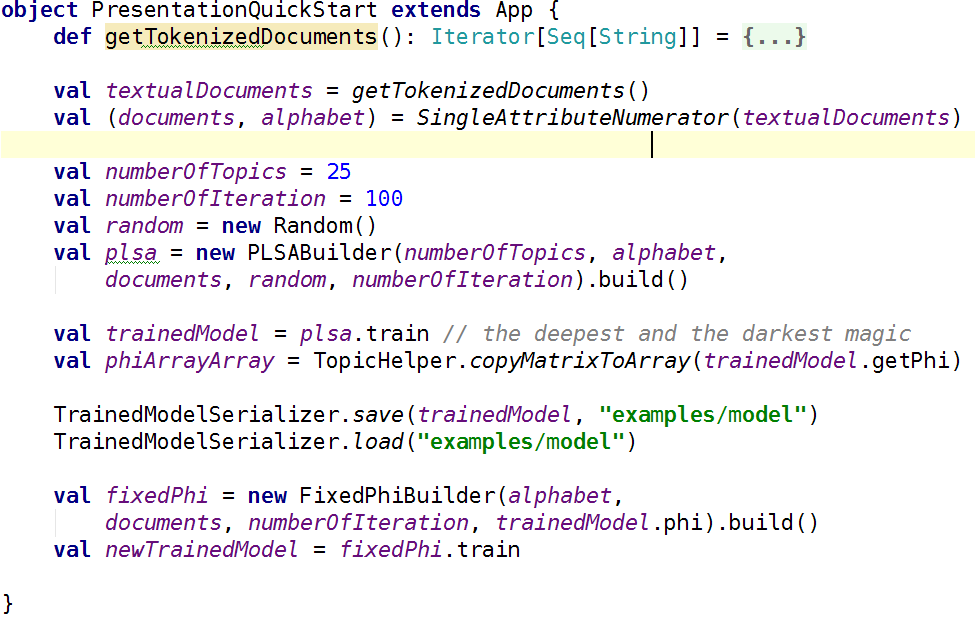
\includegraphics[width=110mm]{quckstart}
	\label{overflow}
    \end{figure}
\end{frame}

\begin{frame}{Счётчики и вероятности}
    \begin{block}{EM-алгоритм}
	\begin{itemize}
	    \item Считаются $n_{dwt}$
	    \item Затем $\phi_{wt} \propto \sum_d n_{dwt}  $ и $\theta_{td} \propto \sum_w n_{dwt}$
	\end{itemize}
    \end{block}
    \begin{block}{Почему стоит объединить матрицу счётчиков и матрицу вероятностей}
	\begin{itemize}
	    \item матрицы счетчиков $n_{w t}$ и $n_{d t}$ и соответствующие матрицы вероятностей $\Phi$ и $\Theta$ связаны по смыслу
	    \item Матриц вероятностей много, но каждой соответствует своя матрица счётчиков
	    \item Матрица счётчиков бесполезна без своей матрицы вероятностей
	    \item Матрица вероятностей бесполезна без  матрицы счётчиков 
	    \item Необходимо ограничить возможность изменения матрицы вероятностей, так чтобы она оставалась нормированной.
	\end{itemize}	
    \end{block}
\end{frame}

\begin{frame}{Огр}    
    \begin{block}{Огры}
	Огр \-- двухголовое создание.\\
	Головы огра это матрица счётчиков и матрица вероятностей\\
	$\Phi$ и $\Theta$ \-- огры
    \end{block}
    \begin{block}{Что огр умеет?}
	\begin{enumerate}
	    \item Хранить матрицу счётчиков и матрицу вероятностей.
	    \item Изменять матрицу счётчиков
	    \item Перемещать значения из матрицы счётчиков в матрицу вероятностей
	    \item Разреживать матрицу вероятностей
	\end{enumerate}	
    \end{block}

    \begin{block}{Зачем это надо}
	\begin{enumerate}
	    \item Счётчики и вероятности всегда вместе, не перепутаешь
	    \item Матрица вероятностей всегда нормирована на 1.	    
	\end{enumerate}	
    \end{block}  
\end{frame}

\begin{frame}{Регуляризаторы}
    \begin{block}{$+R(\Theta, \Phi)$}
	\begin{itemize}
	    \item более человекопонятные темы
	    \item частичное обучение
	    \item LDA
	    \item все что вы хотите
	\end{itemize}
    \end{block}

    \begin{block}{ЕМ-алгоритм}
	$$ \theta_{dt} \propto\sum_d n_{dwt}   + \theta_{dt}\frac{\partial R}{\partial \theta_{dt}} (\Theta, \Phi) $$
	$$\phi_{wt} \propto \sum_d n_{dwt} + \phi_{wt}\frac{\partial R}{\partial \phi_{wt}} (\Theta, \Phi)$$
    \end{block}
\end{frame}

\begin{frame}{Интерфейс}
    \begin{figure}[ht!]
	\centering
	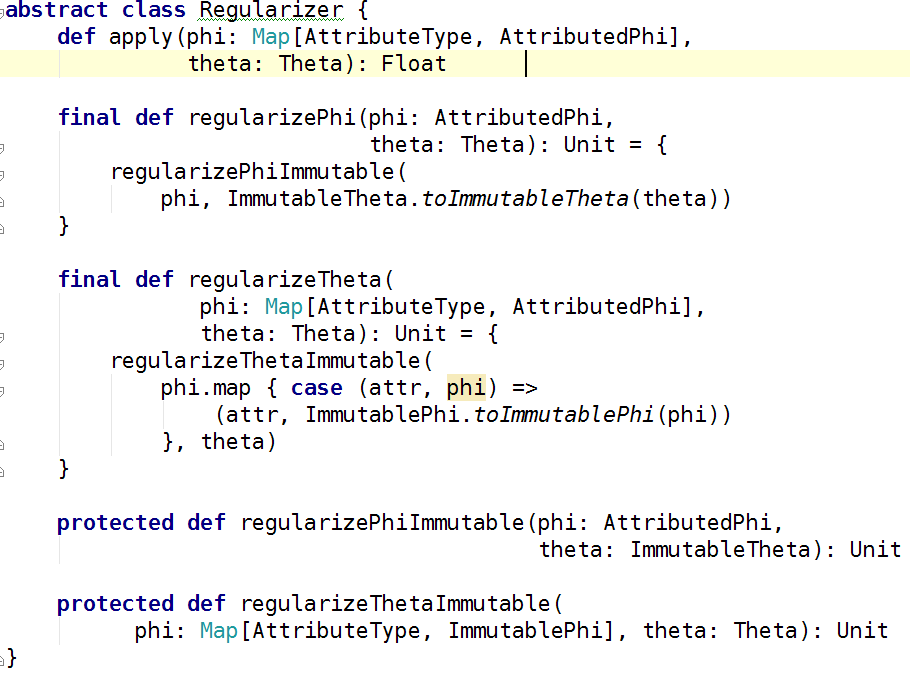
\includegraphics[width=105mm]{regularizer}
	\label{overflow}
    \end{figure}
\end{frame}


\begin{frame}{Разреживатели}
    \begin{block}{Но зачем?}
	Есть мнение, что каждый документ и каждое слово относятся не ко всем темам.

	\texttt{def apply(matrix: MatrixForSparsifier, numberOfIteration: Int): Unit}
    \end{block}

    \begin{block}{\texttt{ MatrixForSparsifier ?}}
	Единственный изменяющий состояние метод --
	\texttt{def setZero(rowIndex: Int, columnIndex: Int)}
    \end{block}
\end{frame}

\begin{frame}{ Генераторы начального приближения}
    \begin{block}{Рандомом плохо?}
	\begin{enumerate}
	    \item Да, плохо
	    \item Невыпуклость задачи
	    \item Быстрее сходится, лучше максимум
	\end{enumerate}
    \end{block}

    \begin{block}{Варианты}
	\begin{enumerate}
	    \item Рандом
	    \item Равномерно (fixed $\phi$)
	    \item Гиббсом
	\end{enumerate}
    \end{block}
\end{frame}


\begin{frame}{Cобираем всю братию вместе}
    \begin{figure}[ht!]
	\centering
	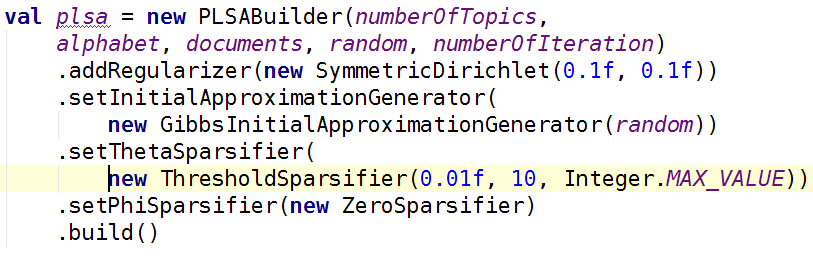
\includegraphics[width=115mm]{builderConfugration.png}
	\label{overflow}
    \end{figure}
\end{frame}



\begin{frame}{Многоязыковость и не только}
    \begin{block}{Было}
	$$d = (w_1 .... w_n )$$
	$$z_{di} \sim \theta_{d \cdot} ~~~~ w_{di} \sim \phi_{z_{di} \cdot }$$
	$$L(\Phi, \Theta) = \sum\limits_{d \in D} \sum\limits_{w \in d}
	    n_{dw} \ln \sum\limits_{t \in T} \phi_{wt}\theta_{td} \rightarrow \max\limits_{\Phi, \Theta}$$
    \end{block}

    \begin{block}{Стало}
	$$d = (w^1_1 .... w^1_{n_1} ), (w^2_1 .... w^2_{n_2} ) , ... (w^l_1 .... w^l_{n_l} ) $$
	$$z_{di^l} \sim \theta_{d \cdot} ~~~~ w_{di}^l \sim \phi_{z_{di} \cdot }^l$$
	\begin{equation*}
	    \begin{split}
		L(\Phi_1, \Phi_2, \Theta) = \sum\limits_{(d_1,d_2) \in D}  \sum\limits_{w \in d^1}
			n_{dw} \ln \sum\limits_{t \in T} \phi^1_{wt}\theta_{td} + \\
			\sum\limits_{w \in d^2}
			n_{dw} \ln \sum\limits_{t \in T} \phi^2_{wt}\theta_{td}  \rightarrow \max\limits_{\Phi, \Theta}
	    \end{split}
	\end{equation*}
    \end{block}
\end{frame}


\begin{frame}{Менее формальное определение}
    \begin{block}{Документы и атрибуты}
	В отличие от обычного тематического моделирования в мультиязычной тематической модели каждому документу может соответствовать несколько текстов, например на разных языках.\\
	При этом распределение по темам у всех документов общее. 
	
    \end{block}

    \begin{block}{Вот как это выглядит:}
	en $\to$ "integral, gradient, matrix" \\ ru $\to$ "матрица, градиент, производная, логарифм", \\ pl $\to$ "пшеИнтеграл, пшеМатрица, пшеПеременная "
    \end{block}
\end{frame}


\begin{frame}{Как это реализовано?}
    \begin{block}{атрибуты}
	\begin{itemize}
	    \item Каждому языку ставится в соответствие свой атрибут. (Word("ru"), Word("en")...)
	    \item Каждый текстовый документ создаётся как\\ Map(атрибут $\to$ текст)
	    \item Каждому атрибуту ставится в соответствие своя матрица $\Phi$ (слова/темы), матрица $\Theta$ (документы/темы) общая. 
	    \item Отображение слов в порядковый номер и наоборот своё для каждого атрибута, но хранится всё в классе $Alphabet$
	\end{itemize}
    \end{block}

    \begin{block}{Не хочу использовать атрибуты}
	Если вы используете только один атрибут, то, по умолчанию используется DefaultAttributeType. \\
	Как всё это выглядит смотри в PresentationQuickStart
    \end{block}
\end{frame}

\begin{frame}{Лепим многоязыковые документы}
    \begin{figure}[ht!]
	\centering
	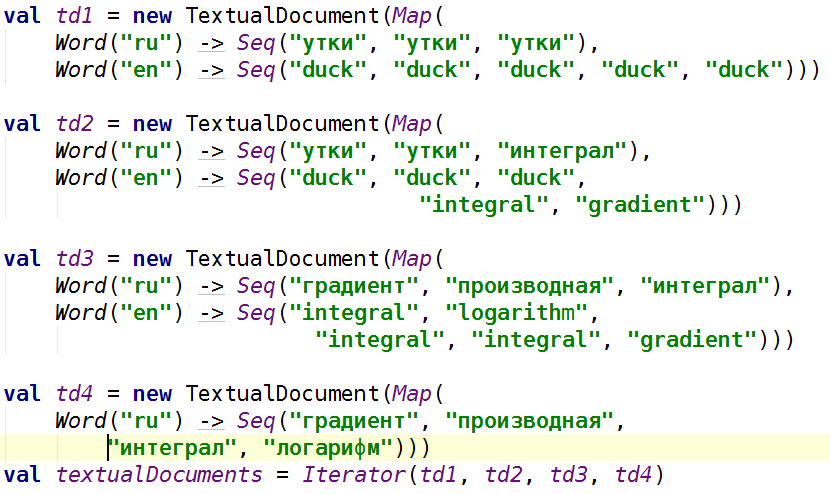
\includegraphics[width=105mm]{multilingualQS}
	\label{overflow}
    \end{figure}
\end{frame}


\begin{frame}{Обучаемся}
    \begin{figure}[ht!]
	\centering
	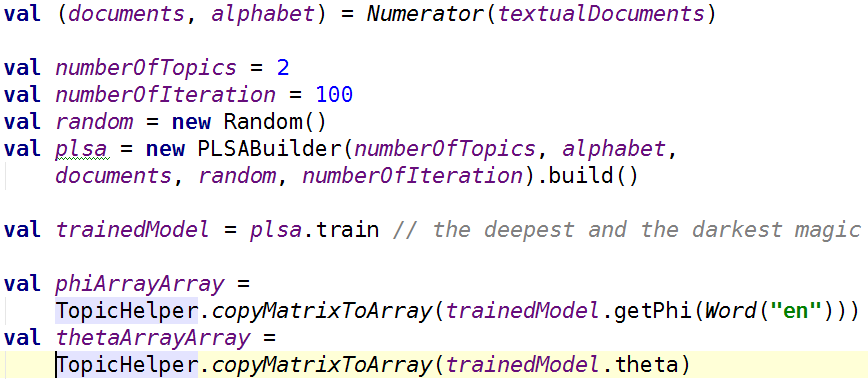
\includegraphics[width=105mm]{multilingualQS1}
	\label{overflow}
    \end{figure}
\end{frame}


\begin{frame}
    \begin{center}
	\Huge Спасибо за внимание!
    \end{center}
\end{frame}


























\end{document}